%! Author = kucera-lukas
%! Date = 4/13/22

\section{Uživatel}\label{sec:uzivatel}

\subsection{Registrace}\label{subsec:registrace}
Na adrese \url{https://stegoer.netlify.app/account?form=register} (pokud není
uživatel již přihlášen) se zobrazí stránka, pomocí které je možné si založit
nový uživatelský účet.

\subsubsection{Náležitosti údajů}\label{subsubsec:naleziosti-udaju}

\begin{enumerate}
    \item Uživatelské jméno musí mit alespoň 6 znaků.
    \item Email musí odpovídat regulernímu výrazu \verb/^\S+@\S+\.\S+$/.
    \item Heslo musí mít minimálně 6 znaků, obsahovat číslo, velké písmeno, malé
    pismeno a alespoň jeden specialní znak.
\end{enumerate}

\subsubsection{Zadávání hesla}\label{subsubsec:zadavani-hesla}

Při vyplnování pole pro heslo se zobrazí popover\cite{enwiki:popover},
který uživateli davá najevo zda jeho heslo splňuje potřebné podmínky.

\begin{figure}
    \centering
    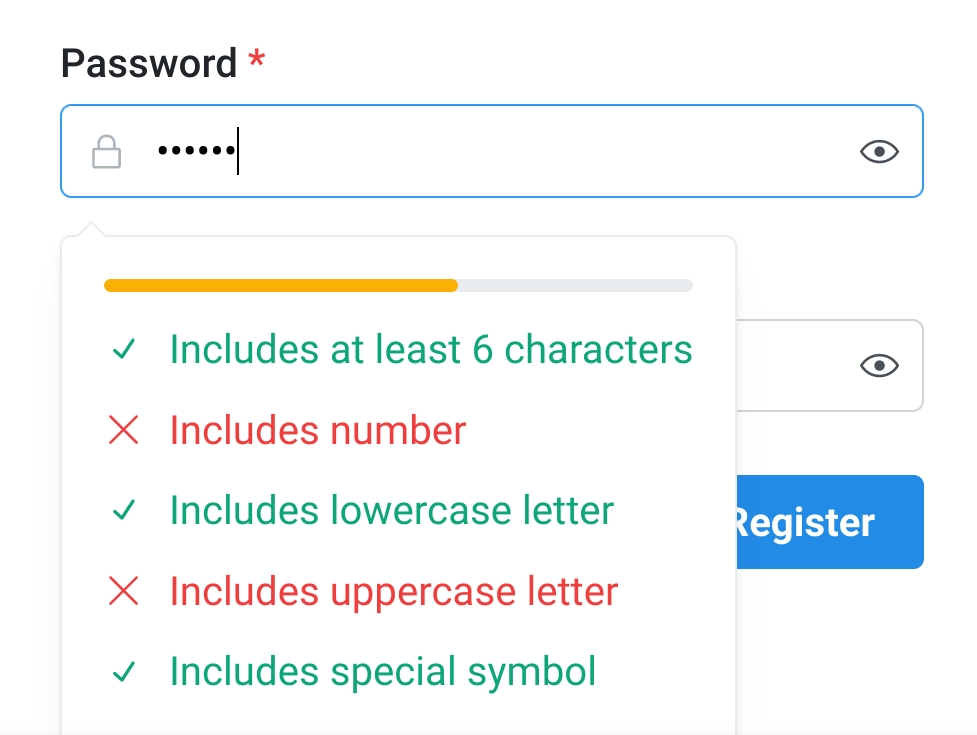
\includegraphics[scale=0.3]{assets/images/password-popover}
    \caption{Zadávaní hesla}\label{fig:zadavani-hesla}
\end{figure}

\subsection{Přihlášení}\label{subsec:prihlaseni}
Na adrese \url{https://stegoer.netlify.app/account?form=login} se zobrazí
přihlašovací stránka.

Zde se pomocí emailu a hesla lze se přihlásit do vlastního účtu (pokud není
uživatel již přihlášen).

U přihlaseni probíhá validace pouze emailu, který by opět měl odpovídat
regulernímu výrazu \verb/^\S+@\S+\.\S+$/.

\subsection{Správa účtu}\label{subsec:sprava-uctu}
Při každém vstupu na adresu \url{https://stegoer.netlify.app/account} aplikace
zkontroje stav uživatele.

Pokud uživatel není přihlášen aplikace ho přesměruje na přihlašovací
stránku\ref{subsec:prihlaseni}.

\subsubsection{Informace o účtu}

Z jednoduché tabulky, která se zobrazí hned při vstupu lze vyčíst tři informace:

\begin{enumerate}
    \item Poslední datum prihlasené uživatele
    \item Poslední datum aktualizace uživatele
    \item Datum vytvoření uživatelského účtu
\end{enumerate}

\subsubsection{Aktualizace účtu}

Pravé tlačítko \texttt{Update account} otevře dialog pomocí kterého může
uživatel zaktualizovat svůj účet.

\paragraph{Změna jména a emailu}

Nabízí se změna uživatelského jména, emailu a i hesla.
Samozřejmě musí být splněny stejné podmínky jako při
registraci\ref{subsec:registrace}.

\paragraph{Změna hesla}

Nabízí se změna uživatelského jména, emailu a i hesla.
Samozrejmě musí byt splněny stejné podmínky jako při
registraci\ref{subsec:registrace}.

\subsubsection{Odhlášení}

Po stisknutí levého tlačítka \texttt{Logout} se uživatel má možnost ze svého
účtu ohlásit.

\subsection{Tabulka obrázků}\label{subsec:tabulka-obrazku}
Na adrese \url{https://stegoer.netlify.app/images} nalezneme tabulku, pomocí
které může uživatel procházet obrázky, do kterých v minulosti uložil nějaká
data.

\begin{figure}
    \centering
    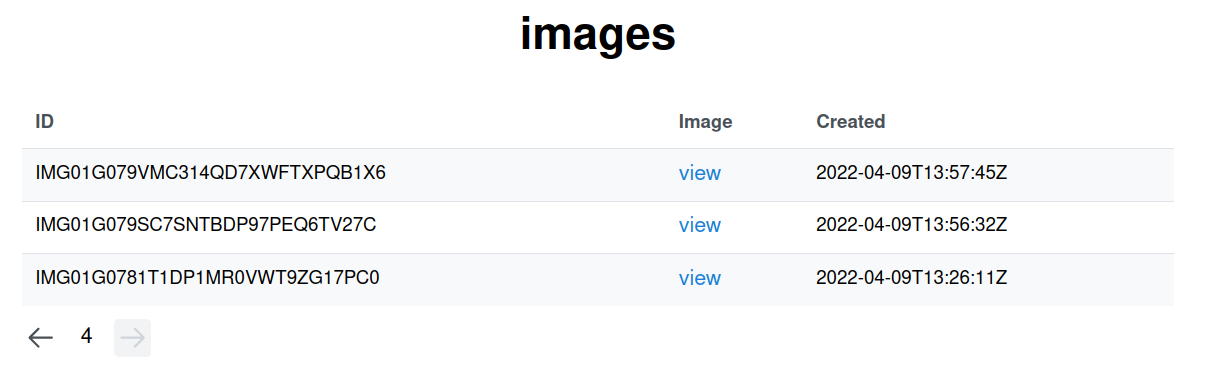
\includegraphics[scale=0.5]{assets/images/images-table}
    \caption{Tabulka s obrázky}\label{fig:tabulka-obrazky}
\end{figure}

\subsubsection{Stránkovani}\label{subsubsec:strankovani}
Na jedné straně se zobrazí maximálně 10 řádku, pro zobrazení ostatních je třeba
použít navigační tlačítka pod tabulkou.

Každý řádek tabulky reprezentuje jeden obrázek a lze z něho vyčíst jeho ID a
datum vytvoření.

\subsubsection{Detail obrázku}\label{subsubsec:detail-obrazku}
Tlačitko \texttt{view}, které se nachází na každém řádku slouží k otevřeni
detailní informace o souboru a možnost si soubor opět znovu stáhnout
(pokud tak uživatel například neučinil po zakódováni dat).

\begin{figure}
    \centering
    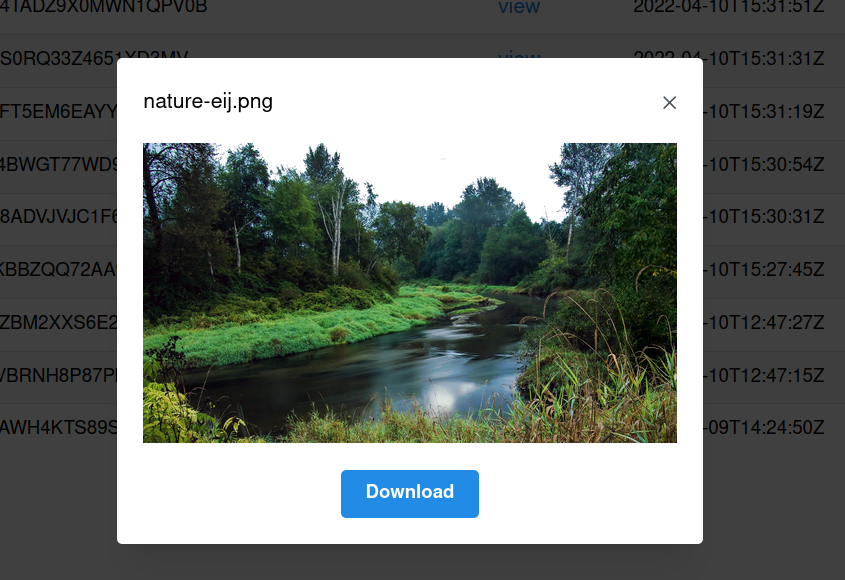
\includegraphics[scale=0.5]{assets/images/image-detail}
    \caption{Detail obrázku}\label{fig:detail-obrazku}
\end{figure}
